\documentclass{article}
\usepackage[utf8]{inputenc}
\usepackage{amsmath}
\usepackage{amsfonts}
\usepackage{amssymb}
\usepackage{graphicx}
\graphicspath{ {./} }

\title{Applied category theory, 18.S097 at MIT. }
\author{Pawan Sasanka Ammanamanchi }
\date{November 2019}
\renewcommand{\thesection}{\Roman{section}.} 
\renewcommand{\thesubsection}{\arabic{section}.\arabic{subsection}}
%\theoremstyle{plain}
\newtheorem{thm}{Theorem}[section] % reset theorem numbering for each chapter

%\theoremstyle{definition}
\newtheorem{defn}[thm]{Definition} % definition numbers are dependent on theorem numbers
\newtheorem{exmp}[thm]{Example} % same for example numbers
\begin{document}


\maketitle
\newpage
\tableofcontents
\newpage
\section{Chapter 1}
\subsection{Lecture 1}
Category theory is a fundamental part of mathematics, it has branched out into a variety of subjects like computer science and physics. Applied category theory is a relatively new field. 
\subsubsection{Generative/ Cascade effects}
A set of different objects while might be observed to not have any common interactions, but when looked at differently might interact with each. Eg: contagion.
\begin{defn}
A set is a bag of dots. 
\begin{equation*}
    A = \{ a,b,c \} \quad where, a, b, c \in A
\end{equation*}
\end{defn}
Similarly, there are different sets of numbers :\\
\\
    $\mathbb{N}, \quad the\, set\, of\, natural\, numbers \\$
    $\mathbb{Z}, \quad the\, set\, of\, integers \\$
    $\mathbb{R}, \quad the\, set\, of\, real\, numbers \\$
    $\mathbb{B}, \quad the\, set\, of\, booleans $ 
    
\begin{defn}
 Product Sets: Suppose A, B are sets then, \\
 \begin{equation*}
     A * B = \{ (a ,b) \mid a \in A, b \in B \} \\
 \end{equation*}
\end{defn} 
In category theory, we think of objects in terms of the roles they play. 
\begin{defn}
 A relation, R,  on sets A and B is defined by\\
 \begin{equation*}
     R \subset A * B \\
 \end{equation*}
\end{defn}
Every function is a relation. Properties like order, equivalence and tolerance are relations as well. 
\begin{defn}
 A function, f, from A to B, denoted $f: A \rightarrow B$ is a relation on A and B. $R \subset A * B$, satisfying 
 \begin{itemize}
     \item For all $a \in A$, there exists an element $b \in B$ such that $(a, b) \in R$. \\
     \item For all a, b1, b2, if $(a, b1) \in R$ and $(a, b2) \in R$, then $b1 = b2$. \\ 
\end{itemize}
\end{defn}
Definition of injective (no two x'es are mapped to the same y) and surjective (for every y there exists an x in the mapping) functions. \\

We can order partitions, Say we have two partitions P1 and P2, then we say 
$P1 \leq P2$ if there is a function $P1 \rightarrow P2$ making the diagram commute.
\begin{figure}
    \centering
    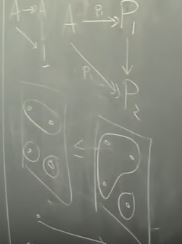
\includegraphics{./images/1.jpg} 
    \caption{When is a partition lesser than another partititon}
    \label{fig:my_label} 
%\end{figure}
%\begin{figure}
    \centering
    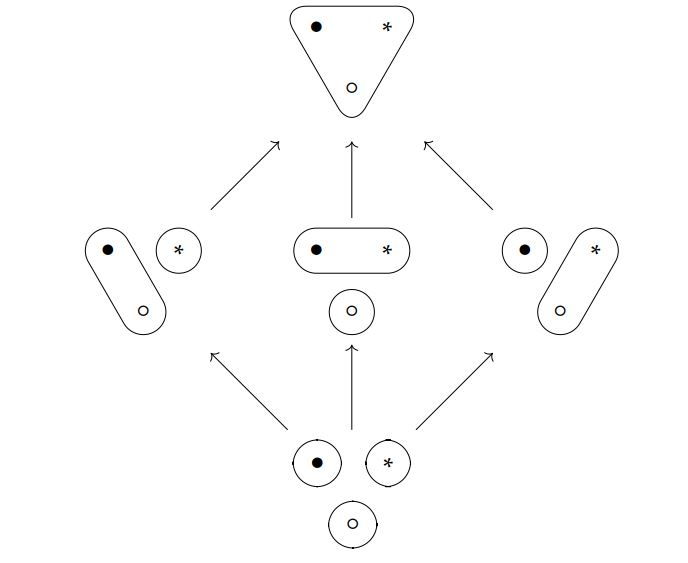
\includegraphics[scale=0.5]{./images/2.jpg} 
    \caption{Can be thought of as a lattice theory structure/ poset}
    \label{fig:my_label}
\end{figure}
\newpage
\noindent
A \emph{pre-order} is 
\begin{enumerate}
    \item a set S
    \item a relation "$\leq$" $\subset S* S$
\end{enumerate}
and also satisfying two properties i.e its reflexive and transitive. 
\newline
Order creates join. 
\subsection{Lecture 2}
Starting with the definition of pre-order, pre-order's are also called posets, A pre-order happens to be a fundamental thing to categories. 
A preorder is a category with at most one morphism between any two objects.
\\
A preorder is a Bool-enriched category. 
\subsubsection{Meets and joins}
Preoder's enable meet and join. 
\begin{defn}
Let $A \subset P$, then $p \in P$ is $a \emph{meet} of A $if
 \begin{itemize}
     \item For all $a \in A$, $p \leq a$. \\
     \item For all $q \in P$, such that for all $a \in A, q \leq a, q \leq p$. \\ 
\end{itemize}
\end{defn}
A meet is the greatest lower bound. Similarly, a join is the least upper bound. 

In elementary boolean logic, the truth table of meet would correspond to AND and the truth table of join would correspond to OR. 

Consider a lattice of power sets, {youtube video: 12:20}, meet is equal to intersection, and join is equal to union. 

Similar notions between preorder and set theory.

When you consider natural numbers as an order with less than to as the relation, then the meet is the minimum and the join is the maximum. When you consider natural numbers as an order with relation, $a \leq b$ if a/b then the meet is the greatest common divisor and the join is the lowest common multiple. 
\newline
\emph{Remark 1}:  Meets/joins may not always exist. A set might not have a meet, if it doesnt have a lower bound. For example, the set of even integers, there is no lowest upper bound i.e the join does not exist. 
\newline
\emph{Remark 2}: Multiple meets/joins might exist. For example, an isomorphic point.  

\subsubsection{Monotone Maps}
\begin{defn}
A monotone map $f: (P, \leq) \rightarrow (q, \leq)$ is a function. 
       $f: P \rightarrow Q$
      such that if $p \leq_p p'$ in P, then $f(p) \leq_q f(p')$ in Q.
\end{defn}

Example, The tree of life. 
When you take the example of lion(species), panthera(genus), carnivore, mammal(class), and sapiens(species), homo(genus) then you see even though there are two preorders, there's a universal map( given below) which connects them. 

$Species \rightarrow Genus \rightarrow Family \rightarrow order \rightarrow class \rightarrow phylum \rightarrow kingdom$.

Cardinality is a monotone map. Contagion under Boolean is a monotone map. 
\begin{figure}[h!]
    \centering
    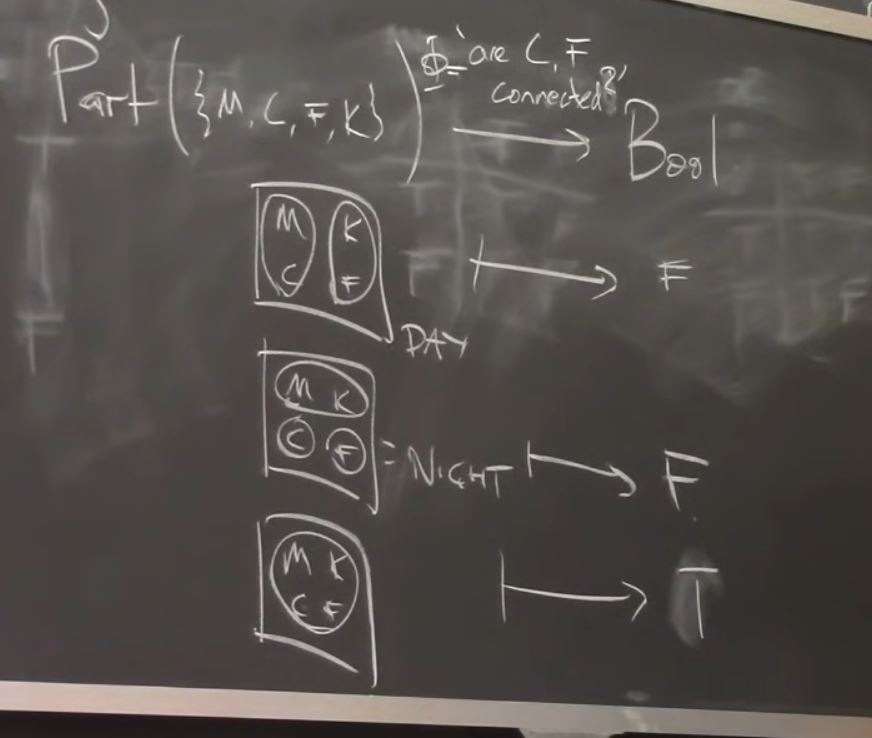
\includegraphics[scale=0.5]{./images/3.jpg} 
    \caption{Contagion under boolean is a monotone map.}
    \label{fig:my_label} 
\end{figure}

\begin{defn}
A monotone map $ f: P \rightarrow Q $ preserves joins \\
if $A \subset P$, $f(\vee A)$ = $\vee \{ f(a)| a\in A \} $
\end{defn}

\emph{Remark:} A monotone map will preserve order, but the universal things like meet and join need not be preserved.
\newpage
\subsubsection{Galois Connections}
\begin{defn}
A galois connection is a pair of posets p and q and monotone map f from p to q and a monotone map g from q to p, i.e

Given P, Q are preorders and f, g are monotone maps such that, 

$ \forall p \in P, q \in Q $ \\
$ f(p) \leq q$ iff $p \leq g(q) $

where f is the left adjoint and g is the right adjoint. 
\end{defn}

\begin{figure}[h!]
    \centering
    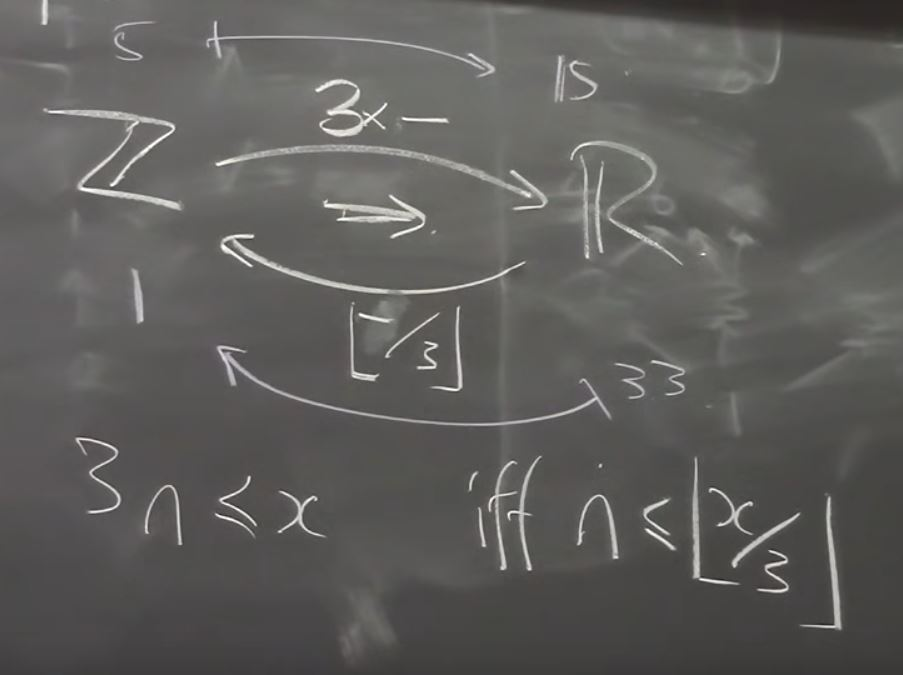
\includegraphics[scale=0.5]{./images/4.jpg} 
    \caption{Example of a galois connection}
    \label{fig:my_label} 
\end{figure}
 
 You'll see throughout these notes, that there are these abstract/ universal constructions and you see some sort of important structure follow through. For example, In the above example of figure 4, the floor is a structure that follows because of the structure given in the left adjoint. 
 
 \begin{defn}
 Adjoint functor theorem for preoders: A monotone map f is a left adjoint iff it preserves joins. A monotone map g is a right adjoint iff it preserves meets. 
 \end{defn}

Adjunctions are also called Galois connections. Meet and joins, products and unions, Discrete Topological spaces, 
Free groups, Group rings, Polynomial rings are all adjunctions in category theory. Meets and joins come under posets
as discussed in the first chapter. But the rest fall under category theory. 

\subsection{Additional Chapter Notes}
In category theory we want to keep control over which aspects of our system are being preserved under various observations. \\
Category theory is all about organizing and layering structures. \\
Given that A is a set, there is a one to one correspondence between the ways to partition A and the equivalence relation on A. \\
\emph{Remark:} Partial orders are sketal preorders. A preorder is a partial order if in addition to reflexivity and transitivity, we also have that $x \cong y$ implies $x = y$. \\

In category theory the aforementioned condition is called skelatality, hence partial orders(poset) are skeletal preorders. All posets are preorders and preorders can be made posets y equating any two elements x,y for which $ x \cong y$ i.e for which $x \leq y $ and  $y \leq x$.





\newpage
\section{Chapter 2}
\subsection{Lecture 1}
\subsubsection{Monoidal posets} 
Monoidal posets -> (Order + combining).
The motivation is to understand resource theories. Resource theories revolve around the fundamental question, "Can i make what i want from what i have?"

\begin{figure}[h!]
    \centering
    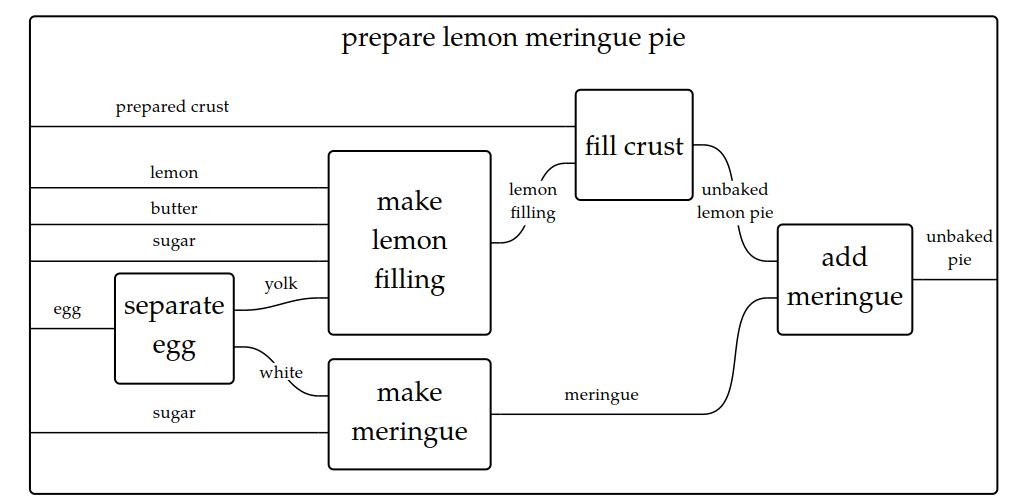
\includegraphics[scale=0.5]{./images/5.jpg} 
    \caption{Resource Theories}
    \label{fig:my_label}
\end{figure}

\begin{defn}
    A monoidal set (A monoid): It consists of a set $M$, a  function $ * : MxM -> M $ and an element $e \in M$
    satisfying \\
    $ (a *b ) * c = a* (b*c) $\\
    $ a * e = a = e * a$
\end{defn}

\begin{defn}
    A monoidal poset: It consists of a poset $M$, a monotone function $ * : MxM -> M $ and an element $e \in M$
    satisfying \\
    $ (a *b ) * c = a* (b*c) $\\
    $ a * e = a = e * a$ \\
    If $a \leq b$ and $c \leq d$, then $a*c \leq b*d$
\end{defn}
Examples: ($\mathbb{N}$, +, 0), ($\mathbb{N}$, * , 1). \\
(Note : Order of the monoidal function space) \\

Can also talk about monoidal spaces, monoidal categories, monoidal abelian group ( a ring) and a monoidal topological space.
\newpage

\subsubsection{Wiring Diagrams(String Diagrams)}
These diagrams involve the human visual cortex. \\
There are varieties of wiring diagrams, As shown in the figure below.

\begin{figure}[h!]
    \centering
    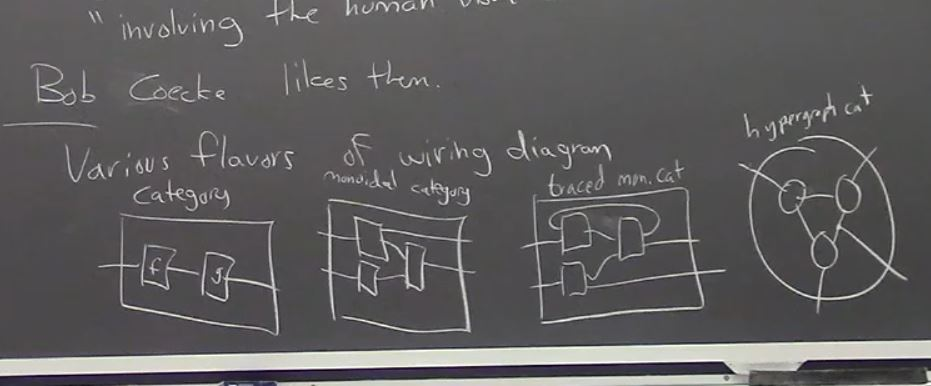
\includegraphics[scale=0.5]{./images/6.jpg}
    \caption{Wiring diagram types}
    \label{fig:my_label}
\end{figure}
Examples from science (Wiring diagrams)
\\
Chemistry examples : \\
$H_2O + H_2O + Na + Na \rightarrow 2NaOH + H_2$
(Petri Nets, Baez) \\
Manufacturing : Add discard axiom. 
Note : Discard axiom in monoids : $\forall a \in M, a \leq e$ \\
\\
Informatics : Add copy axiom. 
Note : Copy axiom in monoids : $\forall a \in M, a \leq a*a$
\\ 
\newpage
\subsection{Lecture 2}
\begin{defn}
    A monoidal prorder $(P, \leq, e, *)$ is
     - a preorder $(P, \leq)$
     - a function $*: P *P \rightarrow P$
     such that, \\
     (a) The * operation is associative \\
     \\(b) * is unital, i.e there exists an identity element. 
     \\(c) if $a \leq c$, $b \leq d$ $\Rightarrow$ $ a*b \leq c*d$.
\end{defn}
Example :
Bool = $({T, F}, \Rightarrow, T, )$ \\
Cost = $([0, \inf], \geq, 0, +)$\\
P(x) = $(P(x), \subset, X, \cap)$\\

\begin{figure}[h!]
    \centering
    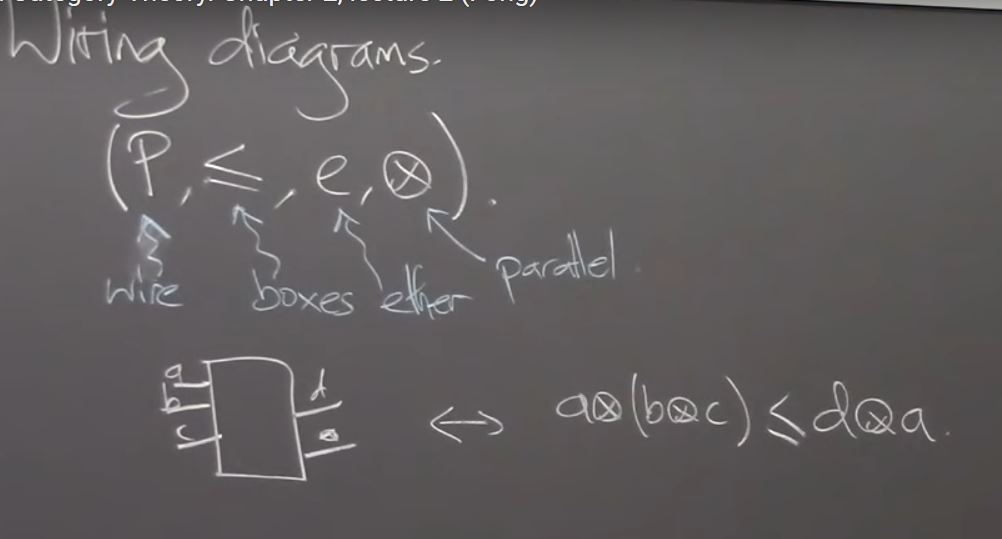
\includegraphics[scale=0.5]{./images/7.jpg}
    \caption{Wiring Diagram Notation}
    \label{fig:my_label}
\end{figure}

\subsubsection{Symmetric Monoidal preorder} 
\begin{defn}
    Symmetric if it obeys: \\
    $a*b \leq b*a$ (symmetric)
\end{defn}



\end{document}


